%This is my super simple Real Analysis Homework template

\documentclass{article}
\usepackage[left=.8in,right=.8in,top=1in,bottom=1in]{geometry}
\newcommand{\reals}{{\mbox{\bf R}}}
\newcommand{\dom}{{\mbox{\bf dom}}}
\newcommand{\var}{{\mbox{\bf var}}}
\newcommand{\E}{{\mbox{\bf E}}}
\newcommand{\tr}{{\mbox{\bf tr}}}
\newcommand{\prob}{{\mbox{\bf prob}}}

\usepackage[utf8]{inputenc}
\usepackage[ruled,vlined]{algorithm2e}

\usepackage{listings}
\usepackage{xcolor}

\definecolor{codegreen}{rgb}{0,0.6,0}
\definecolor{codegray}{rgb}{0.5,0.5,0.5}
\definecolor{codepurple}{rgb}{0.58,0,0.82}
\definecolor{backcolour}{rgb}{0.95,0.95,0.92}

\lstdefinestyle{mystyle}{
    backgroundcolor=\color{backcolour},   
    commentstyle=\color{codegreen},
    keywordstyle=\color{magenta},
    numberstyle=\tiny\color{codegray},
    stringstyle=\color{codepurple},
    basicstyle=\ttfamily\footnotesize,
    breakatwhitespace=false,         
    breaklines=true,                 
    captionpos=b,                    
    keepspaces=true,                 
    numbers=left,                    
    numbersep=5pt,                  
    showspaces=false,                
    showstringspaces=false,
    showtabs=false,                  
    tabsize=2
}

\lstset{style=mystyle}


\usepackage[makeroom]{cancel}
\usepackage{graphicx}
\usepackage{hyperref}

\usepackage[utf8]{inputenc}
\usepackage[english]{babel}
\usepackage[]{amsthm} %lets us use \begin{proof}
\usepackage[]{amssymb} %gives us the character \varnothing
\usepackage{amsmath}
\usepackage{fancyhdr}

\pagestyle{fancy}
\fancyhf{}
\rhead{Tuguluke}
\lhead{CSCI 5254  Homework 6}
\rfoot{Page \thepage} 

\title{CSCI 5254  Homework 6}
\author{Tuguluke Abulitibu}
\date{\today} 
%This information doesn't actually show up on your document unless you use the maketitle command below

\begin{document}
\maketitle %This command prints the title based on information entered above
\section*{Chapter 7, Estimation}	
\subsection*{7.3}
Since $v$ is a zero mean unit variance Gaussian variable, we have the CDF (from sum to integral, since integral is convex):
\[{\displaystyle \Phi (x)={\frac {1}{\sqrt {2\pi }}}\int _{-\infty }^{x}e^{-t^{2}/2}\,dt}\]
in our case:
\[\begin{cases}
\prob(x|y=1) = \dfrac{1}{\sqrt{2 \pi}}\int_{x}^{\infty}e^{\frac{-z^2}{2}}dz\\
\prob(x|y=0) = 1 - \dfrac{1}{\sqrt{2 \pi}}\int_{x}^{\infty}e^{\frac{-z^2}{2}}dz
\end{cases}\]
hence the likely function\footnote{$\prod_{i=1}^q p_i \prod_{i=q+1}^m(1- p_i) $} is 
\[\prod_{i=1}^{q}P_i(a^Tu_i+b|y=1)\prod_{i=q+1}^{m}(1-P_i(a^Tu_i+b|y=0))\]
taking the log:
\[l(a,b) = \sum_{i=1}^{q}\\log(P_i(a^Tu_i+b|y=1))+\sum_{i=q+1}^{m}\log(1-P_i(a^Tu_i+b|y=0))\]
\[\boxed{l(a,b) = \sum _{y_i=1}\log P_i(a^Tu_i+b)+\sum_{y_i=1}\\log(1-P_i(a^Tu_i+b))}\]
objective is concave, hence the problem is convex.
\subsection*{7.4 (a)}
\[-\frac{N}{2}n\log(2\pi)-\frac{N}{2}\log(\det R)- \frac{1}{2}R^{-1}\sum_{k=1}^{N}(y_k-a)(y_k-a)^T\]
\[ = -\frac{N}{2}n\log(2\pi)-\frac{N}{2}\log(\det R)- \frac{1}{2}R^{-1}(\sum_{k=1}^{N}y_ky_k^T-\sum_{k=1}^{N}ay_k^T-\sum_{k=1}^{N}y_ka^T+Naa^T)\]
plug in sample mean $\mu = \dfrac{1}{N}\sum_{k = 1}^n y_k$, we have 
\[= -\frac{N}{2}n\log(2\pi)-\frac{N}{2}\log(\det R)- \frac{1}{2}R^{-1}(\sum_{k=1}^{N}y_ky_k^T-Na\mu^T-N\mu a^T+Naa^T)\]
\[=-\frac{N}{2}n\log(2\pi)-\frac{N}{2}\log(\det R)- R^{-1}\sum_{k=1}^{N}(y_k-\mu)(y_k-\mu)^T-R^{-1}N(a-\mu)(a-\mu)^T\]
plug in covariance $Y  = \dfrac{1}{N}\sum_{k=1}^N (y_k - \mu)(y_k - \mu)^T$, we have 
\[-\frac{N}{2}n\log(2\pi)-\frac{N}{2}\log(\det R)- \frac{1}{2}(NR^{-1}Y + R^{-1}N(a-\mu)(a-\mu)^T)\]
that is the equivalent 
\[ = \dfrac{N}{2}(-n\log(2\pi)-\frac{N}{2}\log(\det R)- \tr(R^{-1}Y) - (a-\mu)^TR^{-1}(a-\mu))\]

Next, by letting
\[\begin{cases}
 \dfrac{\partial}{\partial a } l(R,a) = -2R^{-1}(a-\mu)= 0 \\
  \dfrac{\partial}{\partial R } l(R,a) = -R^{-1} + R^{-1}(Y - (a-\mu)(a-\mu)^T)R^{-1}= 0
  \end{cases} \Rightarrow \begin{cases}
a_{ml} = \mu\\
R_{ml}  = Y  \end{cases}
\]
\subsection*{7.8}
We order values with $y>1$ followed by $y<0$, hence 
\[\prod_{i=1}^{k}\prob(a_i^Tx + b_i + v_i > 0)\prod_{i=k+1}^{m}\prob(a_i^Tx + b_i + v_i < 0)\]
Since the  relative variance is the noise term $v_i$\footnote{$a_i, b_i$ are known}, we introduce CDF F for $\prob$:
\[\prod_{i=1}^{k}F(-a_i^Tx-b_i)\prod_{i=k+1}^{m}1-F(-a_i^Tx-b_i) 
\]
from 7.3, we know that the log-likeihood function is concave
\[l(x) = \sum_{i=1}^{k}\log (F(-a_i^Tx-b_i))+\sum_{i=k+1}^{m}\log (1-F(-a_i^Tx-b_i))\]
therefore maximize problem will be concex\footnote{Textbook page 358:Therefore, for any maximum likelihood estimation problem with concave log likelihood function, we can add a prior density for x that is log-concave, and the esulting MAP estimation problem will be convex.}.
\subsection*{7.9}
$f'(t) > 0$, then it is a monotone function, hence, $f$ is invertible, then from
\[ y_i = f(a_i^Tx +b_i +v_i), i=1,\dots,m\]
 we can get 
 \[v_i = f^{-1}(y_i)-a_i^Tx-b_i\]
 hence the probability of $y_i$ is 
 \[\prod_{i=1}^{m}\prob(f^{-1}(y_i)-a_i^Tx-b_i)\]
 the log-likelihood function will be
 \[l(x, f) = \sum_{i=1}^{m}\log(\prob(f^{-1}(y_i)-a_i^Tx-b_i))\]
 since $f' \in [l, u]$, we know that $f^{-1} \in [1/u, 1/l]$, we get to the convex optimization of ml:
     \[   \begin{array}{ll}
    \mbox{maximize}   &\sum_{i=1}^{m}\log(\prob(f^{-1}(y_i)-a_i^Tx-b_i))\\
    \mbox{subject to} & \dfrac{\|y_i -y_j\|}{u} \le \|f^{-1}_i - f^{-1}_h \| \le  \dfrac{\|y_i -y_j\|}{l}
        \end{array} 
  \]   
introducing $z = f^{-1}$
     \[  \boxed{  \begin{array}{ll}
    \mbox{maximize}   &\sum_{i=1}^{m}\log(\prob(z_i-a_i^Tx-b_i))\\
    \mbox{subject to} & \dfrac{\|y_i -y_j\|}{u} \le \|z_i - z_j \| \le  \dfrac{\|y_i -y_j\|}{l}
        \end{array} 
   }
  \]   
\section*{Chapter 8, Extremal volume ellipsoids}	
\subsection*{8.16}
first of all, we know
\[v = \prod_{i=1}^{n}(u_i-l_i)\]
then maximizing the volume can be maximizing 
\[\prod_{i=1}^{n}(u_i-l_i)^{\frac{1}{n}}\]
this is geometric means, hence concave. \\
Now we can express $x_i$ as $u_i, l_i$, hence
\[\sum_{i=1}^{n}a_{ij}(u_j-l_j) \le b_i\]
by introducing 
\[\begin{cases}
a_{ij}^+  = \max \{a_{ij}, 0\}\\
a_{ij}^- = \max \{-a_{ij}, 0\}\
\end{cases}
\]
we can rewrite the system as 
\[\sum_{i=1}^{n}(a_{ij}^+u_j-a_{ij}^-l_j) \le b_i\]
the max volume problem then become
\[\begin{array}{ll}
    \mbox{maximize}   &(\prod_{i=1}^{n}(u_i-l_i))^{1/n} \\
    \mbox{subject to} & \sum_{i=1}^{n}(a_{ij}^+u_j-a_{ij}^-l_j) \le b_i, \; \forall i
      \end{array} 
\]
 taking the log, we have 
      \[  \boxed{  \begin{array}{ll}
    \mbox{maximize}   &\log(u_i-l_i))^{1/n} \\
    \mbox{subject to} & \sum_{i=1}^{n}(a_{ij}^+u_j-a_{ij}^-l_j) \le b_i, \; \forall i \\
    & u_i \succeq l_i  \; \forall i
        \end{array} 
   }
  \]   
  
\section*{Chapter 8, Classification}	
\subsection*{8.24}
Since \[(a+u)^Tx_i \ge b \Leftrightarrow a^Tx_i+||u||_2|x_i||_2 \ge b\]
and $\|u\|_2 \le \rho$, we have
\[a^Tx_i+\rho\|x_i\|_2 \ge b \Leftrightarrow  \rho \le \dfrac{a^Tx_i - b}{\|x_i\|_2}\]
same for 
\[(a+u)^Ty_j \le b \Leftrightarrow a^Ty_j-b \le -\rho \|y_j\|_2 \Leftrightarrow  \rho \le \dfrac{  b -a^Ty_i}{\|y_i\|_2} \]
this is to say that weight error can be 
\[\min \{ \dfrac{a^Tx_i - b}{\|x_i\|_2} ,  \dfrac{  b -a^Ty_i}{\|y_i\|_2} \}\]
now, introducing auxiliary variable $t$, the weight error margin problem(maximizing the margin) can be written as 
  \[  \boxed{  \begin{array}{ll}
    \mbox{maximize}   &t \\
    \mbox{subject to} & a^Tx_i - b \ge t \|x_i\|_2\;  i = i, \cdots, N \\
     & b -a^Ty_i \ge t \|y_i\|_2\;  j = i, \cdots, M \\
     & \| a\|_2 \le 1
        \end{array} 
   }
  \]   
  

\section*{Additional Exercises}
\subsection*{5.12 Least-squares with some permuted measurements}
Estimate an initial $\hat{x}$ using the huber penalty function. We then use that $\hat{x}$ to calculate a $\hat{P}$ by aligning the indices of $Ax$ and $y$ to find a permutation matrix.  Repeat until the euclidean norm of the distance between the $\hat{x}_{\tau}$ and $\hat{x}_{\tau-1}$ is below  tolerance, then stop.\\

\begin{algorithm}[H]
\SetAlgoLined
 initialization \\
 $x(0) \leftarrow \arg_x \|Ax -y\|$\;
 \Repeat{$P(t) = P(t-1)$}{
   $P(t) \leftarrow \arg max \|Ax(t) - P^Ty\|_2$ \\
    $x(t+1) \leftarrow \arg max \|Ax - P(t)^Ty\|_2$ \\
    Stop if $\|x(t-1) - x(t)\|_2 \le \epsilon$
\;
 }
 \caption{Least-squares with some permuted measurements}
\end{algorithm}
\[ \begin{cases}
 \|x_{true} - x_{naive}\|  = 2.2683660401079058\\
 \|x_{true} - x_{final}\|  = 0.08421494480703208 
\end{cases}
\]
 \lstinputlisting[language=python]{prob512.py}
  \begin{figure}[h!]
\begin{center}
  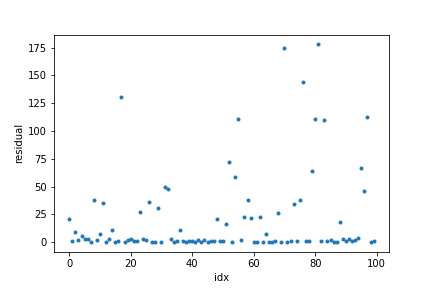
\includegraphics[width=.4\linewidth]{prob_152.png}
\end{center}
\caption{Estimator residual.}
\end{figure}
\subsection*{5.18  Multi-label support vector machine}
\subsubsection*{(a)}
Since
\[L(A,b) = \sum_{i =1}^m (1 + \sum_{k \ne y_i}f_k(x_i)   -f_{y_i}(x_i) )\]
we minimize $L(A,b) +\mu ||A||_F^2  $ which is 
 \[  \boxed{  \begin{array}{ll}
    \mbox{minimize}   &\sum_i z_i + \mu ||A||_F^2  \\
    \mbox{subject to} &1+f_k(x_i)   -f_{y_i}(x_i) \leq z_i, \; \forall k \ne y_i\\
    & z_i \ge 0
        \end{array} 
   }
  \]   

\subsubsection*{(b)}

 \lstinputlisting[language=matlab]{prob518.m}
  \begin{figure}[h!]
\begin{center}
  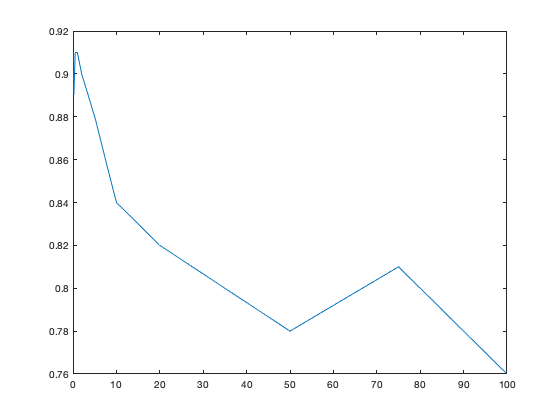
\includegraphics[width=.4\linewidth]{prob518.png}
\end{center}
\caption{Estimator residual.}
\end{figure}\subsection*{6.4 Maximum likelihood prediction of team ability}
\subsubsection*{(a)}
By the CDF def $\Phi(\dfrac{x-u}{\sigma})$,  where $x=y_i(a_{i,j}-a_{i,k})$, we can get the total prob 
\[p(y|a)=\prod_{i=1}^{n}\Phi(\dfrac{y_i(a_i-a_j)}{\sigma})\]
hence the log-likeihood function is 
\[l(a) = \sum_{i}^{n}log(\Phi(\dfrac{y_i(a_i-a_j)}{\sigma}))\]
from here, the problem of finding the maximum likelihood estimate of team abilities is:
 \[  \boxed{  \begin{array}{ll}
    \mbox{maximize}   &\sum_{i}^{n}\log(\Phi(\dfrac{y_i(a_i-a_j)}{\sigma})) \\
    \mbox{subject to} & 0 \preceq a \preceq 1
        \end{array} 
   }
  \]   

\subsubsection*{(b) and (c)}
\begin{verbatim}
Status: Solved
Optimal value (cvx_optval): +11.4487
 

a_hat =

    1.0000    0.0000    0.6829    0.3696    0.7946    0.5779    0.3795    0.0895    0.6736    0.5779


Pml =

  -20.6444
 \end{verbatim} 
 \lstinputlisting[language=matlab]{prob64.m}
\subsection*{6.6 Maximum likelihood estimation of an increasing nonnegative signal}
\subsubsection*{(a)}
    \[  \boxed{  \begin{array}{ll}
    \mbox{minimize}   &\sum_{t=2}^{N+2}(y(t)-\sum_{\tau=1}^{k}h(\tau)x(t-\tau))^2 \\
    \mbox{subject to} & x(N) \ge x(N-1) \ge ... \ge x(1) \ge 0 \\
    & x(t) = 0, t \le 0
        \end{array} 
   }
  \]   

\subsubsection*{(b)}
\lstinputlisting[language=python]{prob66.py}
   \begin{figure}[h!]
\begin{center}
  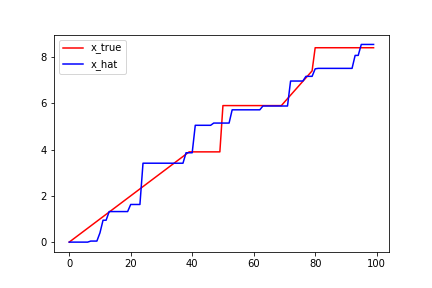
\includegraphics[width=.4\linewidth]{prob_66.png}
\end{center}
\caption{Maximum likelihood estimate $x_{ml}$, along with the true signal.}
\end{figure}
\subsection*{15.3 Utility versus latency trade-off in a network}	
\subsubsection*{(a)}
Maximize the given log (concave) function:
 \[  \boxed{  \begin{array}{ll}
    \mbox{maximize}   &\sum_{j=1}^{n}log(f_j)\\
    \mbox{subject to} & Rf \preceq c,\\
    &  f \succeq 0
            \end{array} 
   }
  \]   
\subsubsection*{(b)}
Latency is the sum of link delays when the link traffic $t_i$ is zero. $d_i = \dfrac{1}{c_i}$ resulting in zero flow. The link delay vector can be written as:
\[(\dfrac{1}{c_1},\dots,\dfrac{1}{c_m})\]
multply by $R^T$ and find the maximum element to get $L^{min}$, we have 
\[L^{min}=\max(R^T(\dfrac{1}{c_1},\dots,\dfrac{1}{c_m})\]
This is to say minimum latency is the maximum of the flow latency.
\subsubsection*{(c)}
Same as part (a), we maximimize the log function, while make sure the latency is min:
 \[  \boxed{  \begin{array}{ll}
    \mbox{maximize}   &\sum_{j=1}^{n}log(f_j)\\
    \mbox{subject to} & Rf \preceq c, f \succeq 0 \\
    & \sum_{i=1}^{m}\dfrac{R_{ij}}{c_i-r_i^Tf} \le L, j=1,\dots,n 
            \end{array} 
   }
  \]   
\subsubsection*{(d)}
 lstinputlisting[language=matlab]{prob157.m}
\end{document}